\documentclass[11pt]{article}
\usepackage{caption}
\usepackage{subcaption}
\usepackage{common}
\pagestyle{plain}
\title{Simulated Annealing and K-Means Clustering to Generate Autonomous Vehicle Pickup and Dropoff Zones}
\author{Jack Stone and Sam Kessler}
\usepackage[htt]{hyphenat}
\usepackage{hyperref}
\newcommand{\code}[1]{\texttt{#1}}

\begin{document}
\maketitle{}


\section{Introduction}

In recent years, ridesharing has greatly simplified the problem of getting from point A to point B in the fastest and cheapest way possible. Though transportation network companies (TNCs) like Uber and Lyft argue that they have had a net positive impact on America`s transportation ecosystem, researchers are sounding alarm bells on some of the darker impacts of TNCs. In particular, evidence is mounting to suggest that ridesharing increases traffic congestion \cite{oecd}. When an Uber car pulls over to wait for a passenger, other cars need to weave around it. This behavior can back up roadways and disrupt the flow of traffic. This has become such a problem in places like airports and hotels that designated pick-up and drop-off zones have begun cropping up at these sites to direct traffic more efficiently. Rather than allowing TNCs to pick up and drop off passengers anywhere they would like, places with drop-off zones only allow drivers to pick up and drop off passengers in spaces which have been specifically allocated for this purpose.

Cities like Boston and San Francisco have already begun thinking  about placing these zones city-wide in order to clear up curb space. Washington, D.C. has even begun running trials evaluating the placement of such zones \cite{oecd}. While the rise of TNCs demands more careful thinking about drop-off zones, these cities are also mindful of the future impact of autonomous vehicles. As more and more vehicles become autonomous, the way we think about transportation and car ownership will change. Most analysts predict that rather than owning their own cars, people (particularly in cities) will increasingly rely upon fleets of autonomous vehicles for their transportation needs \cite{fleets}. Since people will not own cars, they will not need to park them, as AVs run by companies like Uber and Lyft will simply roam around to pick up and drop off passengers. This will reduce the need for parking spaces, but will necessitate the creation of specific pick-up and drop-off zones as more people will be calling rides curbside.

One of the challenges with drop zones is determining where they should be placed. The purpose of our project is to create an algorithm which, given a city map with certain attributes (such as population density), can determine where drop-off zones should be located within that city.


\section{Background and Related Work}

There has not been much prior work devoted to the use of algorithms to intelligently map autonomous vehicle drop-off zones, as this is a relatively new problem. That said, the problem of laying out drop-off zones is somewhat analogous to the problem of arranging bus stops. We did manage to find some interesting solutions to the latter problem. One group of researchers used means clustering, an algorithm somewhat similar to K-Means, to assign bus stops to clumps of houses \cite{busstops}.

\section{Problem Specification}

Given an abstracted city map marked with $N$ ``locations'' (points on the map which have some assigned population density), our goal is to output a new map in which $m$ of the locations are assigned drop zones, or "zones."
\newline

\noindent
Our algorithm should find an arrangement of zones throughout the map such that:
\begin{itemize}
    \item No zone is within $c$ distance of any other zone
    \item No location without a $road$ can contain a zone
    \item Every location on the map is within $d$ distance of the nearest zone
    \item The population density covered by each node is \textit{maximized}
    \item The distance between each zone and each location is \textit{minimized}
\end{itemize}

\section{Approach}

% A clear specification of the algorithm(s) you used and a description
% of the main data structures in the implementation. Include a
% discussion of any details of the algorithm that were not in the
% published paper(s) that formed the basis of your implementation. A
% reader should be able to reconstruct and verify your work from reading
% your paper.

\begin{algorithm}
  \begin{algorithmic}
    \Procedure{SimulatedAnnealing}{$map, old\_cost$}
    \State{$T \gets$ 1.0, the starting value for $T$}
    \State{$T_{min} \gets$ .001, the minimum $T$ value}
    \State{$decay \gets$ .9, the rate of decay}
    \While{$T > T_{min}$}
        \While{$count < 50$}
            \State{$new\_map \gets$ neighbor of $map$, where one drop zone is moved to a random location}
            \State{$new\_cost \gets$ cost of $new\_map$}
            \If{$AcceptanceProbability(old\_cost) > .5$}
                \State{$new\_cost \gets$ $old\_cost$}
                \State{$map \gets$ $new\_map$}
            \EndIf
            \State{$i \gets i + 1$}
            \State{$T \gets T * decay$}
        \EndWhile
    \EndWhile
    
    \Return{$map$}
    \EndProcedure{}
  \end{algorithmic}
  \caption{Simulated Annealing.}
\end{algorithm}

\begin{algorithm}
  \begin{algorithmic}
    \Procedure{KMeansClustering}{}
    \State{$k \gets \text{number of dropoff zones}$}
    \Repeat
        \For{point \textbf{in} points}
            \State{Assign \textit{point} to closest center}
        \EndFor
        \State{}
        \State{Update each center coordinates to the average of its assigned points}
    \Until{No point assignments have changed}
    \EndProcedure{}
  \end{algorithmic}
  \caption{K-Means Clustering.}
\end{algorithm}

We initially considered solving this problem using one of the CSP algorithms discussed in class, but we realized early on that although our problem contains some CSP elements (such as the $road$ binary and the minimum distance constraints), it is more of an optimization problem. Our ultimate approach involved comparing different versions of simulated annealing and K-Means clustering. Simulated annealing starts with a randomly assigned state, and iterates through neighboring states randomly one at a time \cite{annealing}. In this case, a state ($map$) is a map with all $z \in Z$ zones assigned. A neighboring state ($new\_map$) is neighbors with $map$ if all but one of the zones are in the same location. Once it selects a neighboring state, simulated annealing will "accept" that state if it represents an improvement over the previous state. In our case, to check whether a neighbor was an improvement, we used a $cost$ function which took distance to zones and/or population density into account (we tried several such functions, which we describe in the "Experiments" section of this report). If a new state is not an improvement then the algorithm will, with some probability, accept that state anyway. The "acceptance probability" decreases over time, meaning that simulated annealing will begin by jumping between a number of different states before eventually stabilizing and converging to some local minimum or maximum. In this case, because of how we defined our $cost$ function, we searched for a local minimum. K-Means clustering is a different algorithm which gradually clusters a group of nodes into K groups based on proximity to K (increasingly optimum) center points \cite{textbook}. Our K-Means algorithm measured proximity by considering both distance and population density, rather than distance alone.

\section{Experiments}
% Analysis, evaluation, and critique of the algorithm and your
% implementation. Include a description of the testing data you used and
% a discussion of examples that illustrate major features of your
% system. Testing is a critical part of system construction, and the
% scope of your testing will be an important component in our
% evaluation. Discuss what you learned from the implementation.

To evaluate our algorithms, we ran a series of experiments where we varied the cost function and (in the case of simulated annealing) the acceptance probability in order to determine what conditions would best optimize drop zone locations. For each experiment, we started with the same random assortment of drop zones throughout the map, ran our algorithm, and returned the resulting map with the modified drop-zone locations. We evaluated the overall performance of the algorithms by running each of them 100 times, with each experiment in a pass (total passes 100) using the same uniform-random zone distribution for the initial randomized input. We then averaged the costs calculated for each experiment among these 100 runs. Each map was 25x25 in size with 5 zones and 25 city locations.

We scored the algorithms by measuring how well the optimized maps adhered to the problem specification. \textbf{The lower the score, the better.} To score an individual map, we averaged the euclidean distance of each location in the map $n \in N$ from the nearest zone $z \in Z$. We then added these average distances, $minDistance_n$, to the average "scaled population density" of each node: 
$$\frac{minDistance_n}{MAX\_DISTANCE} \cdot density_n$$

where $density_n$ is the population density at node $n$, and $MAX\_DISTANCE$ is a constant representing the maximum distance any location can be from its nearest zone. We scaled the population density in order to take distance into account: the further away a location is from the nearest zone, the less of its population that zone covers, and thus the higher the cost. 
We are left with the following cost function (with $N$ representing the total number of city locations):
$$\text{Cost}(map) = \frac{1}{N}\sum_n \left(minDistance_n + \frac{minDistance_n}{MAX\_DISTANCE} \cdot density_n \right)$$


We evaluated 4 different variations of simulated annealing, each with a different cost function. Version 1 uses a cost function which does not take population into account. Version 2 takes population into account, but does not scale the population (resulting in a higher score, as expected). Version 3 uses the above scoring function, meaning it takes both distance and scaled population density into account, and version 4 is the same as version 3, just with the acceptance probability decreased (meaning it converges much more quickly). We evaluated a single variation of K-Means, where the proximity from a node to a zone takes both distance and density into account (identically to Version 3 of simulated annealing).

The algorithms are detailed below in equation form. Note that $minDistance_n$ represents the euclidean distance between location $n$ and the nearest zone, $distance_{n,z}$ represents the euclidean distance between location $n$ and zone $z$, $density_n$ represents the population density at location $n$, and $MAX\_DISTANCE$ represents the maximum distance that any city location is allowed to be from the nearest drop zone. $N$ is again the total number of city locations.
\newline

\noindent\textbf{Simulated Annealing 1}: Average Distance (Population-Less Cost Function)
$$Cost(map) = \frac{1}{N}\sum_n minDistance_n$$
$$Acceptance\_Probability(old\_cost, new\_cost) = e^{\frac{old\_cost - new\_cost}{T}}$$
\newline

\noindent\textbf{Simulated Annealing 2}: Average Distance + Density (Suboptimal Cost Function)
$$Cost(map) = \frac{1}{N}\sum_n \left(minDistance_n + density_n\right)$$
$$Acceptance\_Probability(old\_cost, new\_cost) = e^{\frac{(old\_cost - new\_cost)/10000}{T}}$$
\newline

\noindent\textbf{Simulated Annealing 3}: Average Distance + Scaled Density (Scoring Function with Biased Acceptance Probability)
$$Cost(map) = \frac{1}{N}\sum_n \left(minDistance_n + \frac{minDistance_n}{MAX\_DISTANCE} \cdot density_n \right)$$
$$Acceptance\_Probability(old\_cost, new\_cost) = e^{\frac{(old\_cost - new\_cost)/10000}{T}}$$
\newline

\noindent\textbf{Simulated Annealing 4}: Average Distance + Scaled Density (Scoring Function w/ Lower Acceptance Probability)
\newline\newline
$$Cost(map) = \frac{1}{N}\sum_n \left(minDistance_n + \frac{minDistance_n}{MAX\_DISTANCE} \cdot density_n \right)$$
$$Acceptance\_Probability(old\_cost, new\_cost) = e^{\frac{old\_cost - new\_cost}{T}}$$
\newline\newline

\noindent\textbf{K-Means}
\newline\newline
\noindent 
$$Distance(n, z) = \frac{distance_{n,z}}{MAX\_DISTANCE} \cdot density_n$$
\newline

\noindent 

\subsection{Results}

Below are the average scores for each algorithm - lower is better. Each algorithm was tested on 100 sample maps with the same initial (uniform) zone distribution.

\begin{center}
  \begin{tabular}{ll}
    \toprule
    & Score \\
    \midrule
    Uniform Distribution & 19926\\
    Sim. Annealing 1 & 14065\\
    Sim. Annealing 2 & 22966\\
    Sim. Annealing 3 & 13642\\
    Sim. Annealing 4 & 13749\\
    K-Means & 13077\\
    \bottomrule
  \end{tabular}
\end{center}

\begin{figure}[h!]
  \centering
  \begin{subfigure}[b]{0.4\linewidth}
    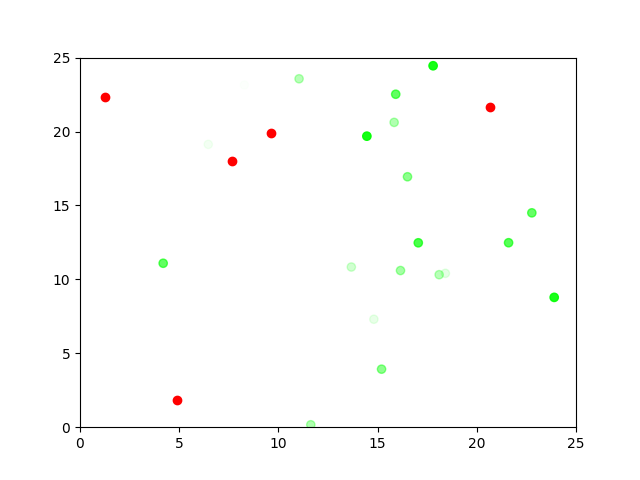
\includegraphics[width=\linewidth]{simulated_annealing_0.png}
    \caption*{Uniformly-distributed zones. Cost: 34393}
  \end{subfigure}
  \begin{subfigure}[b]{0.4\linewidth}
    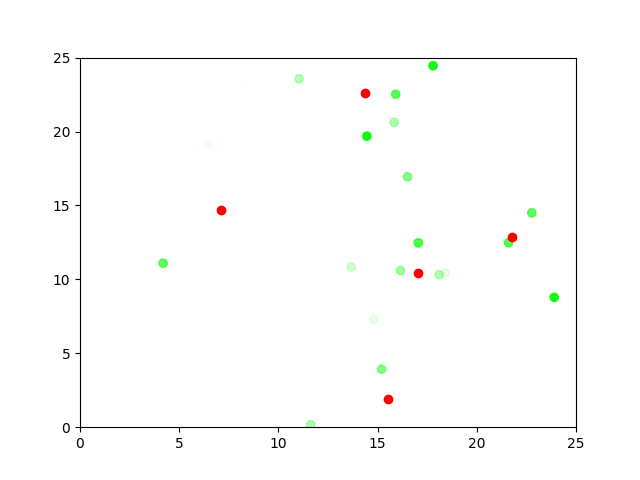
\includegraphics[width=\linewidth]{simulated_annealing_1.png}
    \caption*{Simulated annealing 1. Cost: 12829}
  \end{subfigure}
  \begin{subfigure}[b]{0.4\linewidth}
    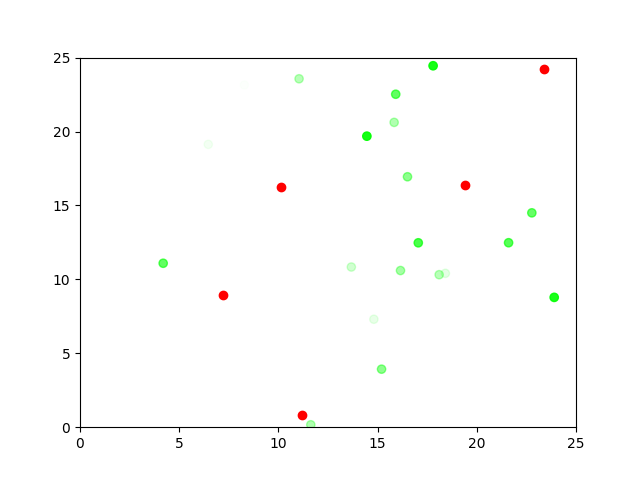
\includegraphics[width=\linewidth]{simulated_annealing_2.png}
    \caption*{Simulated annealing 2. Cost: 23894}
  \end{subfigure}
  \begin{subfigure}[b]{0.4\linewidth}
    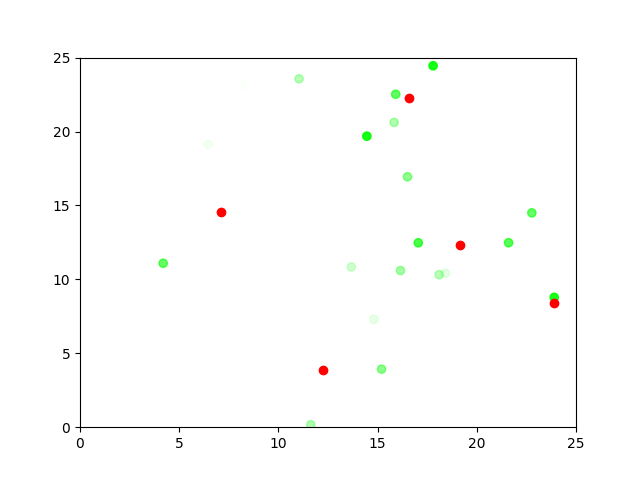
\includegraphics[width=\linewidth]{simulated_annealing_3.png}
    \caption*{Simulated annealing 3. Cost: 12660}
  \end{subfigure}
  \begin{subfigure}[b]{0.4\linewidth}
    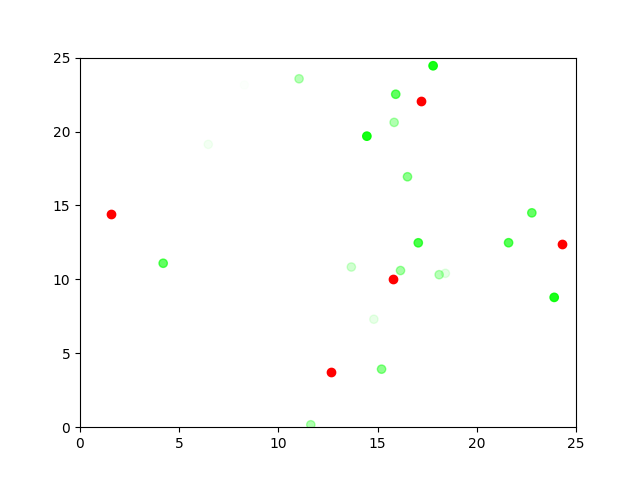
\includegraphics[width=\linewidth]{simulated_annealing_4.png}
    \caption*{Simulated annealing 4. Cost: 13390}
  \end{subfigure}
  \begin{subfigure}[b]{0.4\linewidth}
    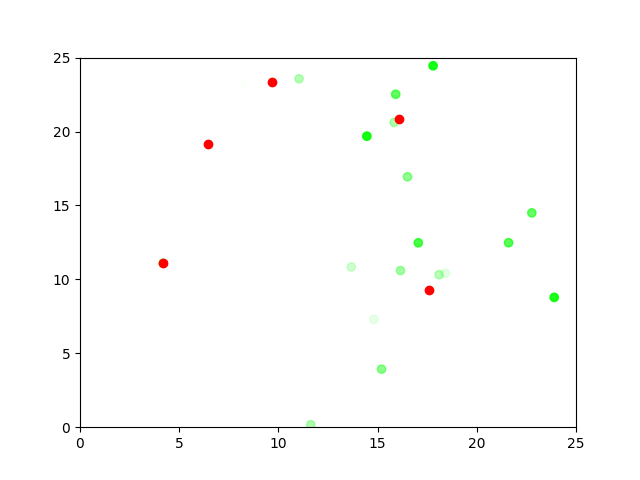
\includegraphics[width=\linewidth]{k_means.png}
    \caption*{K-means clustering. Cost: 16428}
  \end{subfigure}
  \caption{Respective costs calculated from running the simulated annealing and k-means experiments. The x- and y- axes represent where in the city the locations are placed. Red dots represent autonomous vehicle drop zones, and green dots represent city locations, with higher opacities corresponding to higher population density for that location.}
\end{figure}

\begin{figure}[h!]
  \centering
  \begin{subfigure}[b]{0.4\linewidth}
    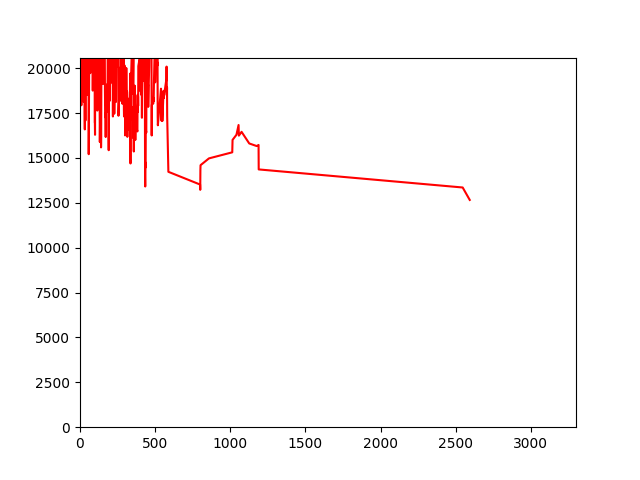
\includegraphics[width=\linewidth]{graph_simulated_annealing_3.png}
    \caption*{Simulated annealing 3}
  \end{subfigure}
  \begin{subfigure}[b]{0.4\linewidth}
    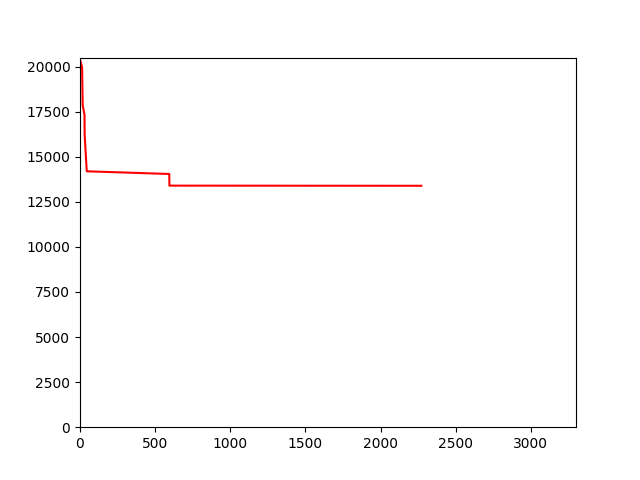
\includegraphics[width=\linewidth]{graph_simulated_annealing_4.png}
    \caption*{Simulated annealing 4}
  \end{subfigure}
  \caption{Graphs of simulated annealing variations 3 and 4. The x-axis represents the time at which the measurement was taken, and the y-axis represents the cost calculated on that iteration.}
\end{figure}
\clearpage

\section{Discussion}

Overall, we have found K-Means clustering to perform slightly better, but similarly to simulated annealing algorithms 3 and 4, which use the same cost function in their acceptance probabilities. In general, all three of these algorithms, in addition to simulated annealing algorithm 1, were vastly superior to naive uniform distributions. Simulated annealing algorithm 2, as expected, was even worse than the uniform distribution, as it always increases the cost by unscaled population, resulting in inflated numbers. It should be noted that, in aggregate, the results appear less striking than they do on an individual level (since the uniform initial distribution of zones does not perform all that poorly for many samples given uniformly-distributed locations). For individual maps where the uniform distribution was scored very poorly, all of these algorithms (except simulated annealing algorithm 2) output maps which were drastically improved relative to the seed maps (which can be seen, for example, in the results from section 5.1). 

It is somewhat surprising that K-Means performs better than simulated annealing versions 3 and 4, since K-Means tends to perform more poorly if given a bad seed. Given that the results for the uniform distribution were relatively low, it is likely that a uniformly-distributed seed distribution of zones tended to match well with the uniformly distributed locations. Perhaps if all of the locations on our maps were assigned using a different distribution, simulated annealing would have performed better than K-Means.

Also somewhat surprising is the fact that simulated annealing algorithms 3 and 4 performed so similarly, despite the fact that simulated annealing algorithm 3 was given significantly more time to bounce between neighbors early on due to the pseudo-normalized acceptance probability. This suggests that the acceptance probability function could have been better-tuned to taper off more gradually. Looking at the time graphs for these two simulated annealing algorithms, the sudden appearance of plateaus in both algorithms suggests that they may have gotten stuck on local minima once the acceptance probabilities dropped near zero. We tried a number of different solutions to make the acceptance probability change more gradually (such as using other normalization constants or dropping/increasing the bias in favor of lower scores), but we failed to arrive at significant enough improvements. Upon reviewing our experiments, one item that we did consider, but did not ultimately have time to implement, was changing the way we classified neighboring states. As we defined it, a neighboring map is one where the location of a single zone has switched locations. For future experiments, we may want to think about specifying a neighboring map as one in which the relevant zone has been moved within a specific radius, rather than any random location on the map. Since moving a zone all the way across the map can significantly increase or decrease cost, it is likely that that this is why our cost jumped around so wildly, even as the acceptance probability decreased. This problem was exacerbated by the fact that our testing maps only contained 5 zones. If we had tried our algorithm on a larger map, we probably would have seen improvements. We also experimented with our decay rate (.9) and minimum T-value (.001), but did not ultimately find this to make much of a difference overall.

Continuing with the topic of the sample maps, another problem with simulated annealing (particularly relative to K-Means) was runtime. Since we were essentially solving a CSP every time we evaluated our cost function, each iteration of the algorithm would take $O(NZ)$ time to evaluate the cost of a given map - looping through each location one by one, and then through each zone to identify which one was closest. Given more time, we would have come up with faster ways of doing this that would have enabled us to test our algorithm on larger maps. For instance, we might have considered breaking the graph into quadrants such that each quadrant was assigned a set number of zones, and we only annealed over one quadrant at a time. Ultimately, a more efficient version of this algorithm would have enabled us to consider more constraints and parameters than we had.

\appendix

\section{System Description}

Please download Python 2.x at \href{https://www.python.org/downloads/}. Before running the project, type \code{pip2 install numpy matplotlib} on the command line to install all relevant Python libraries.

You may then execute the contents of the project by typing \code{python2 algorithm.py}. As it stands now, that command will run 100 passes of simulated annealing and k-means clustering. You may change the number of passes by modifying the \code{num\_passes} variable on line 19 of \code{algorithm.py}. On each pass, the program runs the four variants of simulated annealing followed by k-means clustering, and saves the output of each as both a graph and an x-y plot in the results folder. The naming scheme is \code{simulated\_annealing\_x.png} and \code{graph\_simulated\_annealing\_x.png}, where \code{x} corresponds to the variant of simulated annealing that is represented in the output. Note that \code{simulated\_annealing\_0} represents the initial graph with uniformly distributed drop zones. The k-means output can also be found in the results folder as \code{k\_means.png}. There is no corresponding graph for the k-means algorithm.

For the x-y plot images, the x- and y- axes represent where in the city the locations are placed. Red dots represent autonomous vehicle drop zones, and green dots represent city locations, with higher opacities corresponding to higher population density for that location. For the graphs, the x-axis represents the time at which the measurement was taken, and the y-axis represents the cost calculated on that iteration.

On each pass, the program will print the respective costs for the initial map, the four variants of simulated annealing, and the k-means algorithm. When the program finishes executing, it will print out the average costs over all passes, in the order of initial map, simulated annealing 1, 2, 3, 4, and k-means.

\section{Group Makeup}
The project code can be found at \href{https://github.com/JackStoneDev/cs182-final-project}.
\newline

Sam Kessler's primary responsibility was the writeup, and Jack Stone's primary responsibility was the code, although they both wrote code and wrote the paper. Both members of the group worked equally designing the poster and the algorithms used.


\bibliographystyle{plain} 
\bibliography{project-template}

\end{document}